\documentclass[10pt,preprint]{aastex}

\newcommand{\kms}{\,km~s$^{-1}$}
\def\squig{\sim\!\!}
\newcommand{\Msun}{\mbox{\,$M_{\odot}$}}
\newcommand{\Lsun}{\mbox{\,$L_{\odot}$}}

\PScommands
\newcommand{\graybox}[1]{\psboxit{box 0.7 setgray fill}{\spbox{#1}}}

\newcommand{\mdmlimit}{0.5}
\newcommand{\vmaxmean}{56}
\newcommand{\mrmean}{-14.7}

\newcommand{\latin}[1]{{#1}}
\newcommand{\ie}{\latin{i.e.}}
\newcommand{\eg}{\latin{e.g.}}
\newcommand{\cf}{\latin{c.f.}}
\newcommand{\Sersic}{S\'ersic}
\newcommand{\vv}[1]{{\bf #1}}
\newcommand{\df}{\delta}
\newcommand{\dfft}{{\tilde{\delta}}}
\newcommand{\betaft}{{\tilde{\beta}}}
\newcommand{\erf}{{\mathrm{erf}}}
\newcommand{\erfc}{{\mathrm{erfc}}}
\newcommand{\Step}{{\mathrm{Step}}}
\newcommand{\ee}[1]{\times 10^{#1}}
\newcommand{\avg}[1]{{\langle{#1}\rangle}}
\newcommand{\Avg}[1]{{\left\langle{#1}\right\rangle}}
\def\simless{\mathbin{\lower 3pt\hbox
    {$\,\rlap{\raise 5pt\hbox{$\char'074$}}\mathchar"7218\,$}}} % < or of order
\def\simgreat{\mathbin{\lower 3pt\hbox
    {$\,\rlap{\raise 5pt\hbox{$\char'076$}}\mathchar"7218\,$}}} % > or of order
\newcommand{\iras}{{\sl IRAS\/}}
\newcommand{\petroratio}{{{\mathcal{R}}_P}}
\newcommand{\petroradius}{{{r}_P}}
\newcommand{\petronumber}{{{N}_P}}
\newcommand{\petroratiolim}{{{\mathcal{R}}_{P,\mathrm{lim}}}}
\newcommand{\band}[2]{\ensuremath{^{#1}\!{#2}}}
\newcommand{\Vmax}{\ensuremath{V_\mmax}}
\newcommand{\mmax}{\ensuremath{\mathrm{max}}}
\newcommand{\mmin}{\ensuremath{\mathrm{min}}}
\newcommand{\minmax}{\ensuremath{\mathrm{\left\{^{min}_{max}\right\}}}}
\newcommand{\fixMr}{\ensuremath{M_\fixr}}
\newcommand{\fixr}{\ensuremath{{r}}}
\newcommand{\fixredshift}{0.1}
\newcommand{\fixmag}[1]{\ensuremath{{^{\fixredshift}\!{#1}}}}

\setlength{\footnotesep}{9.6pt}

\newcounter{thefigs}
\newcommand{\fignum}{\arabic{thefigs}}

\newcounter{thetabs}
\newcommand{\tabnum}{\arabic{thetabs}}

\newcounter{address}

\shortauthors{Blanton {\it et al.} (2014)}
\shorttitle{Notes on NSA tests with Simard Catalog}

\begin{document}

\title{Notes on Tests of NASA-Sloan Atlas Fluxes:\\
Tests against Simard GIM2D Models and Measurements}


\author{
Michael R. Blanton\altaffilmark{\ref{NYU}}
}

%\altaffiltext{1}{Based on observations obtained with the
%Sloan Digital Sky Survey\label{SDSS}}
\setcounter{address}{1}
\altaffiltext{\theaddress}{
    \stepcounter{address}
    Center for Cosmology and Particle Physics, Department of Physics, New
    York University, 4 Washington Place, New
    York, NY 10003
    \label{NYU}}

\begin{abstract}
I test the NASA-Sloan Atlas measurements of flux and sizes against
those of \citet{simard11a}, concentrating on galaxies brighter than
$r\sim16.5$. 

First, for galaxies from the \citet{simard11a} catalog, I create a set
of 10,000 simulated images, to which I apply the NSA flux and size
measurement procedure. From these measurements I demonstrate that for
these models Petrosian quantities defined with elliptical apertures,
including the flux and $r_{50}$ values, agree reasonably well with the
intrinsic properties of the models. Within 5\%, the Petrosian fluxes
behave as expected; with about a 20\% underestimate for de Vaucouleurs
galaxies. For galaxies with $r_{50}>2$ arcsec, the Petrosian $r_{50}$
values are slightly lower than the intrinsic values (given the
\citet{simard11a} definition), but within 10--15\% independent of
galaxy properties. Below $r_{50} \sim 2$ arcsec, the Petrosian
$r_{50}$ is always reported as around 2 arcsec, because it is not
corrected for seeing. Circularized Petrosian quantities have several
size-dependent biases that affect them.

Second, I applied the elliptical Petrosian measurements to the
deblended NSA images in the $r$-band.  I match to the
\citet{simard11a} catalog and test the differences between the
analysis techniques for real data. These differences reflect to some
degree the differences seen for the model data. In the elliptical
Petrosian $r_{50}$ relative to the GIM2D measurements, there exists a
trend with size; the Petrosian sizes are 15\% less than the GIM2D
sizes at $r_{50}\sim 10$ arcsec.
\end{abstract}

\setcounter{thefigs}{0}

\section{Code, Data, and Methods} 
\label{sec:code}

These tests were done using the {\tt dimage} software used for the
NASA-Sloan Atlas processing, described in \citet{blanton11a}. This was
work was performed between revisions {\tt r1116} and {\tt r1132} of
that code.

The \citet{simard11a} catalog I used was the pure de Vaucouleurs plus
exponential fit, as downloaded as a FITS file from Vizier. Where
necessary, I matched this to the NSA with a 2 arcsec tolerance. I
trimmed the \citet{simard11a} catalog for the plots to only include
galaxies with $r_{50}>2$ pixels, which eliminated 5-10\% of their
objects; 99\% of the objects smaller than that were stars, based on
the visual inspection of 500 of them.

The NSA data was from {\tt v1\_0\_0}, which includes galaxies up to
$z=0.15$. I reanalyzed the child images for the $r$-band from that
data. The NSA already includes circularized Petrosian quantities as
well as single-component \Sersic\ fits. This data resides on riemann
at:
\begin{center}
{\tt /clusterfs/riemann/raid000/blanton/atlas} 
\end{center}
The {\tt v1\_0\_0} catalog is in the {\tt v1} subdirectory. This is
accessible on the SDSS-III site at:
\begin{center}
{\tt http://data.sdss3.org/sas/ebosswork/manga/atlas}
\end{center}
In particular, the Petrosian fluxes and sizes calculated for the NSA
catalog can be found in the {\tt test/petro} subdirectory.

The Petrosian method tested uses an estimate of an axis ratio $b/a$
(minor over major) and position angle $\phi$ to define a set of
elliptical annuli. Otherwise it uses the standard algorithm for
Petrosian magnitudes, with the Petrosian radius $r_P$ defined as the
semimajor axis of the ellipse where the Petrosian ratio $\eta= I/\bar
I = 0.2$, and with the aperture for the flux defined with a radius
$2r_P$. I measure $r_{50}$ and $r_{90}$ as the ellipses whose the
semimajor axes enclose 50\% and 90\% of the flux within $2r_P$. Within
about 2 pixels the method is approximate; in practice, the Petrosian
radius as usually defined has a radius of 4--5 pixels in SDSS data, so
this is adequate for our purposes here.

Several choices are available for defining $b/a$ and $\phi$. The NSA
determines axis ratios based on second moments within its
(circularized) Petrosian $r_{50}$ and $r_{90}$, as well based on its
single-component \Sersic\ fit. The results I show in this document use
the Petrosian-based axis ratios; however, I impose a lower limit of
$b/a=0.2$.

In detail, the elliptical Petrosian measurement is done with a piece
of python code ({\tt petro.py}) called by an executable script {\tt
  petro2d}. The outputs are put into each atlas image directory next
to the measurement files; they are later gathered into a single file
with {\tt petro2d\_gather}. The calculation takes somewhat less than 1
second per image on average. On riemann, this results in about 10
hours of processing time; this is almost certainly I/O bound when done
in parallel, and I haven't optimized the number of processors to use.

\section{Measuring Petrosian quantities on simulated images} 
\label{sec:models}

To test the code and investigate the reliability of this method in a
controlled environment, I put together a set of 10,000 simulated
images (code used was {\tt simard\_tests.pro}). These images were
based \citet{simard11a} catalog parameters for a randomly selected set
of objects with $r<16.5$, roughly the limit for MaNGA. I created fake
images with roughly the sky noise of SDSS data (around 0.03 nmgy per
pixel in the $r$-band) and with typical-to-good SDSS seeing (a FWHM of
2.84 pixels, or 1.1 arcsec). In detail, the seeing was modeled as a
set of three axisymmetric concentric Gaussians). \citet{simard11a}
provides a model-based definition of half-light ratio, which is to
project each model component onto its major axis (which can differ),
sum the result, and calculate the half-light radius on that sum.

I ran the standard NSA measurement code on each fake galaxy (not
including the \Sersic\ fitting), and then the elliptical Petrosian
measurements. Figures \ref{fig:petro} and \ref{fig:petroc} show the
results for the elliptical and circular Petrosian measurements; in
particular, they show the difference between the measured quantities
and the model quantities as a function of flux, size, and $B/T$
ratio. 

The sizes and fluxes for the elliptical measurements show some
residuals respect to these quantities but are fairly
well-behaved. There are some slight offsets in flux and size, and for
flux there is the well-known dependence of Petrosian flux on
$B/T$. Most of these effects are at the 10\% level; the flux
dependence on $B/T$ is somewhat larger (15--20\%).

The sizes and fluxes for the circularized measurements show greater
residuals and scatter, as expected. Interestingly, there is a strong
dependence the Petrosian $r_{50}$ measurement on size even at large
radii, well above the seeing limit. This dependence is reduced if we
shuffle the overall half-light radii among the models but keep the
other parameters fixed, indicating that the size dependence of the
circularized Petrosian measurement may be associated with a slight
correlation between galaxy angular size and the galaxy's $b/a$ (or in
principle other parameters).
 
\stepcounter{thefigs}
\begin{figure} 
\figurenum{\fignum}
\includegraphics[width=0.49\textwidth]{test-simard-petro-flux-vA.ps} \quad
\includegraphics[width=0.49\textwidth]{test-simard-petro-r50-vA.ps} 
\caption{\label{fig:petro} Comparison between simulated galaxies based
  on \citet{simard11a} models and elliptical Petrosian
  measurements. Sizes and fluxes across most of the range of most
  parameters are within 20\% (and typically closer) of the models. At
  small sizes ($r_{50} < 2$ arcsec) the Petrosian sizes become seeing
  limited. }
\end{figure}

\stepcounter{thefigs}
\begin{figure}
\figurenum{\fignum}
\includegraphics[width=0.49\textwidth]{test-simard-petrocirc-flux-vA.ps} \quad
\includegraphics[width=0.49\textwidth]{test-simard-petrocirc-r50-vA.ps} 
\caption{\label{fig:petroc} Comparison between simulated galaxies based
  on \citet{simard11a} models and circular Petrosian measurements. In
  addition to the seeing limit for Petrosian sizes, at large sizes
  there is a trend of circularized $r_{50}$ with true size for the
  galaxies. This appears to at least partly be due to a correlation
  between the angular size and the profile shapes and/or ellipticities
  in the \citet{simard11a} catalog. }
\end{figure}

\section{Measuring Petrosian quantities on real galaxies} 
\label{sec:real}

I have measured the Petrosian elliptical aperture magnitudes on the
$r$-band delended images of all of the galaxies in the NSA {\tt
  v1\_0\_0} catalog. Figures \ref{fig:realpetro} and
\ref{fig:realpetroc} show the differences between the elliptical and
circular Petrosian measurements and the \citet{simard11a} catalog.

The residuals for the elliptical Petrosian measurements are not as
clean in the real data as for the simulations. The larger overall
scatter is likely due to differences in deblending or sky
subtraction. The feature at $r>16.5$ occurs because I selected the
galaxies by Petrosian $r$ (not the \citet{simard11a} magnitude). 

Other than that, there is a trend of Petrosian $r_{50}$ against the
\citet{simard11a} angular size (middle right panel). At about $r_{50}$
of 10 arcsec, this corresponds to a 15\% median difference in size
(Petrosian less than GIM2D).  I did try a slightly larger aperture for
the Petrosian flux ($2.5r_P$ instead of $2r_P$). This results in a
small (5\%) increase in the typical $r_{50}$, but without affecting
the size dependence. The reason for the residual size dependence is
unclear. One possibility is a difference in the sky-subtraction. A
second is that the galaxy profiles differ from the GIM2D models in a
size-dependent fashion, inducing differences in the Petrosian
quantities or errors in the GIM2D sizes, or both.

The residuals for the circular Petrosian measurements show the
features expected from the simulations. These features are therefore
clearly an artifact of the azimuthal averaging.

For completeness, I show in Figure \ref{fig:realsersic} the
differences between the single-component \Sersic\ quantities and the
\citet{simard11a} measurements for the NSA galaxies. These show very
large residuals.

\stepcounter{thefigs}
\begin{figure}
\figurenum{\fignum}
\includegraphics[width=0.49\textwidth]{simard-petro-flux.ps} \quad
\includegraphics[width=0.49\textwidth]{simard-petro-r50.ps} 
\caption{\label{fig:realpetro} Comparison between \citet{simard11a}
  measurements and elliptical Petrosian measurements for NSA galaxies
  with $r<16.5$.  The residuals seen in the real measurements are
  similar to those seen for the models, but with somewhat more size
  dependence for $r_{50}$.}
\end{figure}

\stepcounter{thefigs}
\begin{figure}
\figurenum{\fignum}
\includegraphics[width=0.49\textwidth]{simard-petroc-flux.ps} \quad
\includegraphics[width=0.49\textwidth]{simard-petroc-r50.ps} 
\caption{\label{fig:realpetroc} Comparison between \citet{simard11a}
  measurements and circular Petrosian measurements for NSA galaxies
  with $r<16.5$.  The residuals seen in the real measurements are
  similar to those seen for the models.}
\end{figure}

\stepcounter{thefigs}
\begin{figure}
\figurenum{\fignum}
\includegraphics[width=0.49\textwidth]{simard-sersic-flux.ps} \quad
\includegraphics[width=0.49\textwidth]{simard-sersic-r50.ps} 
\caption{\label{fig:realsersic} Comparison between \citet{simard11a}
  measurements and single-component \Sersic\ measurements for NSA
  galaxies with $r<16.5$. } 
\end{figure}
 
\bibliographystyle{apj}
\bibliography{../../ccpp-latex/ccpp}

\end{document}
 
